\documentclass[lang=cn, titlestyle=display, scheme=chinese]{elegantbook}

\usepackage{amsmath, bbm, graphicx, enumerate}
\usepackage[math-style=ISO, bold-style=ISO]{unicode-math}
\setmathfont{Garamond-Math.otf}[StylisticSet={7,9}] %设置数学字体
\graphicspath{{assets/images}{assets/logos}} %设置图片路径
\pagenumbering{arbic} %设置页码为阿拉伯数字
%封面设置
\title{数学物理方法简明讲义}
\definecolor{customcolor}{RGB}{32,178,170}
\colorlet{coverlinecolor}{customcolor}
\author{saYmd}
\date{\today}
\version{a2.0}
\cover{cover.png}
\logo{logo.jpg}

\setcounter{tocdepth}{2} %设置目录深度

\begin{document}
    \maketitle
    \tableofcontents
    \frontmatter
    \mainmatter

    \chapter{复微积分}
\begin{introduction}
    \item 复变函数
    \item 解析函数
    \item 多值函数
    \item 复变函数的积分
\end{introduction}
\section{复变函数}
    \subsection{复变函数的定义}
        与实数集上的实变函数相对应,复变函数就是由复数集到复数集的映射.\par
        \begin{definition}[复变函数]\label{def:complex_function}
            对于映射$f: \mathbbm{C} \to \mathbbm{C}$,写作$f(z)=w$,称为复变函数.
        \end{definition}

        复变函数是平面到平面的映射,它将复平面$z$上的点逐一映射到复平面$w$上.
        对于任意复数$z \in \mathbbm{C}$,我们可以将其写作如下形式$z = x + iy,(x,y \in \mathbb{R})$,
        于是我们也可以将复变函数$f(z) = w$写作两个实变函数的形式:
        \begin{align}
            f(z) = u(x,y) + iv(x,y)
        \end{align}

        其中,$u(x,y)$和$v(x,y)$分别是$f(z)$的实部和虚部,点$(u, v)$为复平面$w$上的点.

    \subsection{复变函数的极限}
        \begin{definition}[复变函数的极限]\label{def:limits_of_complex_function}
            极限$lim_{z \to a}f(z) = w_0$表示对于任意实数$\epsilon > 0$,都存在一个实数$\delta > 0$,
            使得当$|z - a| < \delta$时,都有$|f(z) - w_0| < \epsilon$.
        \end{definition}

        \begin{definition}[复变函数的连续性]\label{def:continuity_of_complex_function}
                    同理,在$z = a$处如果有$lim_{z \to a}f(z) = f(a)$,则称$f$在$z = a$处连续.
                \end{definition}


\section{解析函数}

    \subsection{复变函数的微分}
        判断一个复变函数是否可微,我们有Cauchy-Riemann条件:
        \begin{theorem}[Cauchy-Riemann条件]\label{thm:Cauchy-Riemann_condition}
            对于复变函数$f(z) = u(x,y) + iv(x,y)$,如果对于点$z_0$,有
            \begin{align}
                \frac{\partial u}{\partial x} = \frac{\partial v}{\partial y} \quad and \quad \frac{\partial u}{\partial y} = -\frac{\partial v}{\partial x}
            \end{align}
            $f$在$z = z_0$处才能可微.
        \end{theorem}

        注意$Cauchy-Riemann$条件仅是$f$可微的必要不充分条件,这里给出判断$f$可微的充要条件:
        \begin{theorem}\label{thm:differentiability_of_complex_function}
            复变函数$f(z) = u(x, y) + iv(x, y)$在区域$G$上可微的充要条件为,$C-R$条件成立:
            \begin{align*}
                \frac{\partial u}{\partial x} = \frac{\partial v}{\partial y} \quad and \quad \frac{\partial u}{\partial y} = -\frac{\partial v}{\partial x}
            \end{align*}
            且在区域$G$上,$u$和$v$的一阶导存在且连续.
        \end{theorem}

        \begin{proposition}\label{pro:complex_function_differential}
            计算复变函数微分的时候大部分情况下都是直接使用与实变函数相同的求导公式,但当我们进行证明时可能会用到$f(x,y)=u(x,y)+iv(x,y)$的形式,现在给出复变函数微分的另一种形式.
            \begin{align}
                \frac{d f}{d z} &= u_x + iv_x \label{eqa:complex_differential}\\
                &= v_y - iu_y
            \end{align}
            当然我们一般使用式\ref{eqa:complex_differential}的形式.
        \end{proposition}
        \begin{proof}
            由$z=x+iy,\,z^*=x-iy$可得,$x=(z+z^*)/2,\,y=(z-z^*)/2$.
            \begin{align}
                \begin{split}
                &x_z=\frac12,\ y_z=\frac1{2i}.\\
                u_z&=u_x x_z + u_y y_z = \frac12 u_x + \frac1{2i} u_y,\\
                v_z&=v_x x_z + v_y y_z = \frac12 v_x + \frac1{2i} v_y.
                \end{split}
            \end{align}
            当$f(z)$可微时有$C-R$条件成立,即$u_x=v_y,\,v_x=-u_y$.我们可以得到
            \begin{align*}
                \frac{df(u,v)}{dz}&=u_z+iv_z\\
                &=\frac12 u_x + \frac1{2i} u_y+i\left(\frac12 v_x + \frac1{2i} v_y\right)\\
                &=\frac12 (u_x + v_y) + \frac i2 (- u_y + v_x)\\
                &=u_x + iv_x\\
                &=v_y - iu_y.
            \end{align*}
        \end{proof}

        \begin{lemma}
            \label{lem:complex_function_differentiable_with_respect_to_z}
            当$f$可微时,$f$与$z^*$无关,即$\dfrac{df}{dz^*} = 0$.
        \end{lemma}
        \begin{proof}
            这里的证明与命题\ref{pro:complex_function_differential}十分相似,首先$z=x+iy,\,z^*=x-iy\ x=(z+z^*)/2,\,y=(z-z^*)/2i$.
            \begin{align*}
                &x_{z^*}=\frac{1}{2},\quad y_{z^*}=-\frac{1}{2i}.\\
                u_{z^*}&=u_x x_{z^*} + u_y y_{z^*}=\frac{1}{2}(u_x+iu_y),\\
                v_{z^*}&=v_x x_{z^*} + v_y y_{z^*}=\frac{1}{2}(v_x+iv_y).
            \end{align*}
            由于$f(z)=f(u,v)=u(x,y)+iv(x,y)$可微,则有$C-R$条件成立,即$u_x=v_y,\ v_x=-u_y$.\\
            我们可以得到
            \begin{align*}
                \frac{df(u,v)}{dz^*}&=u_{z^*}+iv_{z^*}=\frac{1}{2}(u_x+iu_y)+\frac{i}{2}(v_x+iv_y)\\
                &=\frac{1}{2}(u_x-v_y)+\frac{i}{2}(u_y+v_x)=0
            \end{align*}

        \end{proof}
        由引理\ref{lem:complex_function_differentiable_with_respect_to_z},我们可以给出另外一种判断$f$是否可微的方法:
        \begin{example}
            判断函数$f(z) = x^2 +2iy^2$的可微性
        \end{example}
        \begin{solution}
            我们有:
            \begin{align*}
                x = \frac{1}{2}(z + z^*), \quad y = \frac{1}{2i}(z - z^*)
            \end{align*}
            将$f(z)$使用$z$和$z^*$重写,
            \begin{align*}
                f(z) &= [\frac{1}{2}(z + z^*)]^2 + 2i[\frac{1}{2i}(z - z^*)]^2\\
                &= \frac{1}{4}(1 - 2i)(z^2 + z^{*2}) + \frac{1}{2}(1 + 2i)zz^*
            \end{align*}
            可以看到$f$与$z^*$有关,因此$f$不可微.
        \end{solution}

    \subsection{解析函数的定义}
        \begin{definition}[解析函数]\label{def:analytic_function}
            如果复变函数$f$在某一点$z_0$及其某一领域$U_0$上可微,则称$f$在$z_0$处解析.相应的,
            若$f$在某一区域$G \subset \mathbbm{C}$上均可微,则称$f$在$G$上解析.$f$解析的点称为正则点.
        \end{definition}
        \begin{definition}[奇点]\label{def:singular_point}
            若$f$在某一点$z_0$处不解析,则称$z_0$为$f$的奇点.
        \end{definition}
        \begin{theorem}[Laplace 方程]\label{thm:Laplace_equation}
            若$f$在某一区域$G$上解析,则$f$在$G$上满足拉普拉斯方程:
            \begin{align*}
                \frac{\partial^2 u}{\partial x^2} + \frac{\partial^2 u}{\partial y^2} = 0. \quad \frac{\partial^2 v}{\partial x^2} + \frac{\partial^2 v}{\partial y^2} = 0
            \end{align*}
            由$C-R$条件易得.
        \end{theorem}

    \subsection{初等单值解析函数}
        \allowdisplaybreaks
        \begin{enumerate}
            \item 幂函数$z^n$\\
                当$n = 0,1,2,\dots$时,$z^n$在$\mathbbm{C}$上解析;且当$n = 1,2,\dots$时,$z^n$在$z = \infty$不解析.\\
                当$n = -1,-2,\dots$时,$z^n$在$z = 0$不解析,在包括$\infty$点在内的$\mathbb{C}$上除$0$外均解析.
            \item 多项式函数$P_n(z) = a_nz^n + a_{n-1}z^{n-1} + \dots + a_1z + a_0$
            \item 有理函数$R(z) = \dfrac{P_n(z)}{Q_m(z)}, \quad Q_m \neq 0$
            \item 指数函数$e^z$\\
                复指数函数具有周期性,这是实指数函数所不具有的,其周期为$2 \pi i$\\
                $e^z$在$\mathbb{C}$上解析,且在$z = \infty$不解析,证明如下:
                \begin{proof}
                    当$z$沿正实轴趋于无穷时,有$x \to \infty, \quad y = 0$,则$\lim_{z \to \infty}e^z = \lim_{x \to +\infty}e^x \to +\infty$;\\
                    而当$z$沿负实轴趋于无穷时,有$x \to -\infty, \quad y = 0$,则$\lim_{z \to -\infty}e^z = \lim_{x \to -\infty}e^x \to 0$;\\
                    可得$e^z$在$z = \infty$处不解析.
                \end{proof}
            \item 三角函数$\sin{z}, \cos{z}, \dots$\\
                复三角函数一般使用复指数函数来定义:
                \begin{align*}
                    \sin{z} &= \frac{e^{iz} - e^{-iz}}{2i}, \quad \cos{z} = \frac{e^{iz} + e^{-iz}}{2}
                \end{align*}
                在$z = \infty$处不解析.
            \item 双曲函数$\sinh{z}, \cosh{z}, \dots$\\
                复双曲函数同样由复指数函数定义.
                \begin{align*}
                    & \sinh{z} = \frac{e^z - e^{-z}}{2},& &\cosh{z} = \frac{e^z + e^{-z}}{2}, & \tanh{z} = \frac{\sinh{z}}{\cosh{z}}&\\
                    & \coth{z} = \frac{\cosh{z}}{\sinh{z}},& &\textnormal{sech}\,z = \frac{1}{\cosh{z}}, & \textnormal{csch}\,z = \frac{1}{\sinh{z}}&
                \end{align*}
                并且易知复双曲函数和复三角函数可以互相转化.
                \begin{align*}
                    \sinh{z} = -i\sin{iz}, \quad \cosh{z} = \cos{iz}, \quad \tanh{z} = -i\tan{iz}
                \end{align*}
        \end{enumerate}


\section{多值函数}

    \subsection{多值函数的定义}
        \allowdisplaybreaks
        \begin{definition}[多值函数]\label{def:multi_value_function}
            复数的幅角多值性导致某些函数将$z$平面上的点映射到$w$平面时,一个点会有多个点与之对应,我们就将这样的函数称为多值函数.
        \end{definition}

        事实上多值函数并不是函数,因为函数要求一一映射.我们主要研究的多值函数就是$f(z) = \sqrt{z - z_0}$和$f(z) = \ln{z}$,
        他们俩的多值性由下式给出:
        \begin{align}
            \label{eq:multi_value_function}
            &\sqrt{z - z_0} = \sqrt{|z - z_0|e^{i(\theta + 2n\pi)}} = \sqrt{|z - z_0|}e^{i\frac{\theta}{2}}e^{in\pi} = \pm \sqrt{|z - z_0|}e^{i\frac{\theta}{2}}\\
            &\ln{z} = \ln{|z|} + i(\theta + 2n\pi)
        \end{align}

        \begin{definition}[分支点(枝点)]\label{def:branch_point}
            如果多值函数的自变量$z$绕点$z_0$外任意闭合曲线$C$一圈后,多值函数的宗量(即$f(z) = \sqrt{z - z_0}$中的$z - z_0$)
            相位改变了$2\pi$,则称点$z_0$为多值函数的分支点.
        \end{definition}

        当我们做各种各样的计算时,肯定不希望出现多值的现象,从分支点的特性出发,你或许也能感觉到,只要避免自变量绕着分支点
        一直转圈圈,我们就能避免多值的出现.因此,我们可以通过限制自变量的取值范围来避免多值的出现,这就是多值函数的分支的概念.

    \subsection{黎曼面}
        \begin{figure}[htbp]
            \centering
            \begin{minipage}[t]{0.48\textwidth}
                \centering
                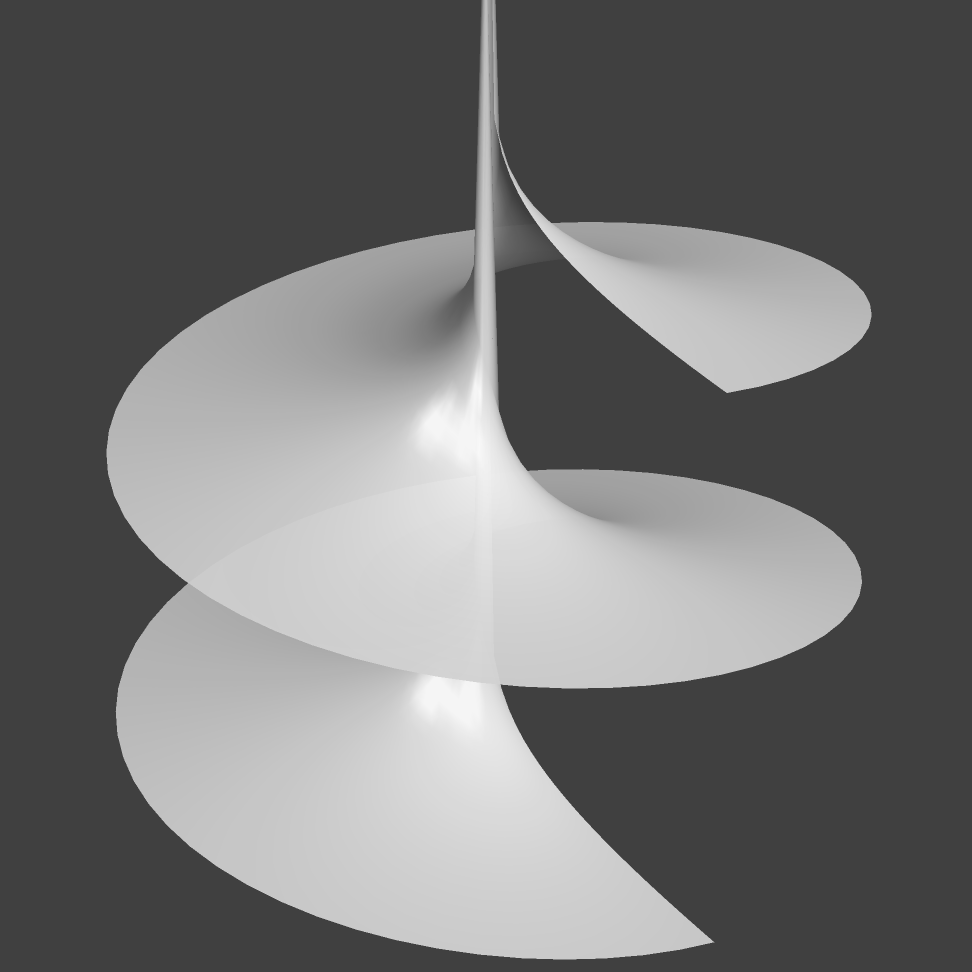
\includegraphics[width=0.9\textwidth]{RiemannSurface.png}
                \caption{$f(z) = \sqrt{z - z_0}$的黎曼面}
                \label{fig:riemann_surface}
            \end{minipage}
            \begin{minipage}[t]{0.48\textwidth}
                \centering
                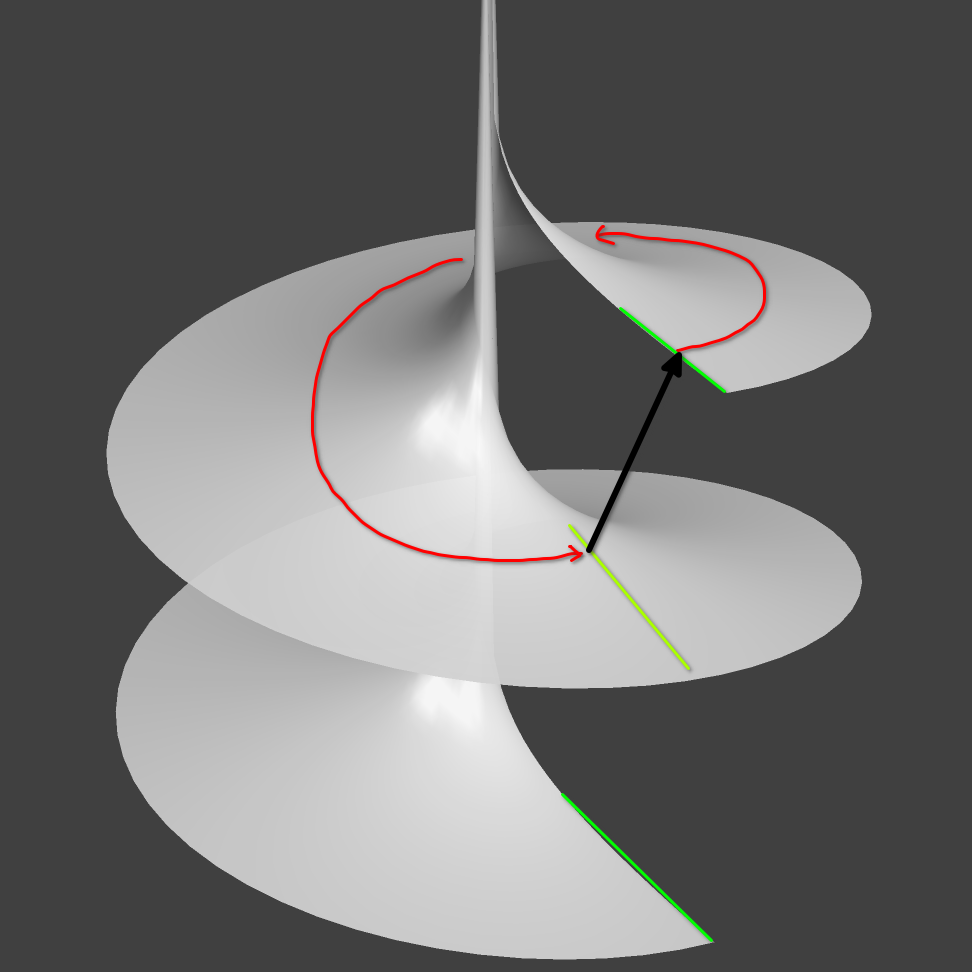
\includegraphics[width=0.9\textwidth]{RiemannSurfacePainted.png}
                \caption{黎曼面上的路径}
                \label{fig:riemann_surface_painted}
            \end{minipage}
        \end{figure}

        黎曼面实际上就是对多值函数定义域的扩充,再看看我们的老朋友$f(z) = \sqrt{z - z_0}$,因为它将点$z$映射到了两个点
        $\pm \sqrt{|z - z_0|}e^{i\frac{\theta}{2}}$上,所以它并不是严格的函数,为了将其变为单值函数,我们只要取两个复平面,
        将定义域铺在这两个复平面上,这样就能避免一对二的情况.

        多值函数$f(z) = \sqrt{z - z_0}$的黎曼面就类似图\ref{fig:riemann_surface}所示,但实际上在三维空间中我们没办法画出黎曼面的准确形状,
        因为你需要用某种神秘力量把图\ref{fig:riemann_surface_painted}中的上下两条绿线粘在一起.

        \begin{definition}[Riemann Sheet]
            黎曼面上的每个平面被叫做黎曼叶(Riemann Sheet),多值函数在单个黎曼叶上是解析的单值函数.图\ref{fig:riemann_surface}中的黎曼面叫做双叶黎曼面,
            因为它是由两个复平面拼接而成的,同理,由几个复平面拼接成的黎曼面就叫做几叶黎曼面.
        \end{definition}

        观察图\ref{fig:riemann_surface_painted},我们让$z$沿红线由三楼向下走,对于多值函数$f(z) = \sqrt{z - z_0}$,
        每当$z$经过一次绿线时,函数值都会加一个负号,而当$z$走到一楼的绿线时,它就会被超时空传送回三楼的绿线处,
        也就是函数值回归到初始值,这就是黎曼面的一个特性,也就是说函数值在黎曼面上是周期的.

        同样,我们也可以很容易地画出$f(z) = \ln{z}$的黎曼面,它和\ref{fig:riemann_surface}差不多,但它是无限叶的,
        每经过一次绿线,函数值都会加(减)一个$2\pi i$.

        \begin{definition}
            若$z$绕分支点$z_0$在黎曼面上旋转$n$圈后,函数值回归初始值,那么我们就将$z_0$称为$n - 1$阶分支点.
        \end{definition}

        \begin{example}
            \label{ex:riemann_surface}
            指出多值函数$f(z) = \sqrt{(z + 1)(z - 2)}$的分支点及其类型.
        \end{example}
        \begin{solution}
            根式的可能分支点在$\infty$和根式内多项式的零点处.
            \begin{enumerate}[(a)]
                \item $z = -1$;在此点领域内任取一点 $z_1 = -1 + \rho_1 e^{i \phi_1}(\rho_1 \ll 1)$,有:
                    \begin{align*}
                        \sqrt{(z + 1)(z - 2)} = \sqrt{\rho_1 e^{i \phi_1}(-3 + \rho_1 e^{i \phi_1})} 
                        \approx \sqrt{-3 \rho_1}e^{i\frac{\phi_1}{2}}
                    \end{align*}
                    当$\phi_1$变为$\phi_1 + 2\pi$,即绕$z = -1$一周时,有:
                    \begin{align*}
                        \sqrt{(z + 1)(z - 2)} \approx \sqrt{-3 \rho_1}e^{i\frac{\phi_1 + 2\pi}{2}}
                        = -\sqrt{-3 \rho_1}e^{i\frac{\phi_1}{2}}
                        \neq \sqrt{-3 \rho_1}e^{i\frac{\phi_1}{2}}
                    \end{align*}
                    而当$\phi_1 + 2\pi$变为$\phi_1 + 4\pi$,即再绕$z = -1$一周时,有:
                    \begin{align*}
                        \sqrt{(z + 1)(z - 2)} \approx \sqrt{-3 \rho_1}e^{i\frac{\phi_1 + 4\pi}{2}}
                        = \sqrt{-3 \rho_1}e^{i\frac{\phi_1}{2}}
                    \end{align*}
                    所以$z = -1$为一阶分支点.
                \item $z = 2$;过程同上,也为一阶分支点
                \item $z = \infty$;在其邻域内任取一点$z_2 = \rho_2 e^{i \phi_2}(\rho_2 \gg 1)$,有:
                    \begin{align*}
                        \sqrt{(z + 1)(z - 2)} \approx \rho_2 e^{i\phi_2}
                    \end{align*}
                    当$\phi_2$变为$\phi_2 + 2\pi$,即绕$z = \infty$一周时,仍有:
                    \begin{align*}
                        \sqrt{(z + 1)(z - 2)} \approx \rho_2 e^{i\phi_2 + 2\pi}
                        = \rho_2 e^{i\phi_2}
                    \end{align*}
                    函数值没有发生改变,所以$z = \infty$不是分支点.
            \end{enumerate}
        \end{solution}

        对于例\ref{ex:riemann_surface}中的函数,我们得到了它的两个分支点$z = -1$和$z = 2$,
        如果我们连接这两个分支点,我们会发现,每当$z$经过这条连线时,$f(z)$就会产生多值性,
        于是我们把这样的线称作割线,只要限制多值函数的自变量始终不越过割线,我们就能保证函数值的唯一性.
        

    \subsection{初等多值函数}
        本小节只作扩展,咱们在多值函数这方面并不会考这么多,只需要掌握根式下多项式形式的多值函数
        (即$\sqrt{(z - a_1)(z - a_2)\cdots(z - a_n)}$)分支点和割线的求法即可.

        \begin{enumerate}
            \item 一般幂函数$w = z^a = e^{a \ln{z}}$
                \begin{enumerate}[(1)]
                    \item 当$a$为整数$n$时,$w$为$z$的单值函数.
                    \item 当$a$为\ 待续... %TODO
                \end{enumerate}
        \end{enumerate}

\section{复变函数的积分}

    \subsection{复积分}
        \begin{definition}[复积分]\label{thm:complex_integral}
            复积分可以简单定义为:
            \begin{align*}
                \int_{\alpha_1}^{\alpha_2}f(z)dz 
                = \lim_{\substack{N \to \infty \\
                \varDelta z_j \to 0}}
                \sum_{j = 1}^{N}f(z_j)\varDelta z_j
            \end{align*}
            其中,$\varDelta z_j$是在$z_j$处的小分割,$z_j$位于连接$\alpha_1, \, \alpha_2$的曲线上.
        \end{definition}

        我们可以将$f(z)$写作$f(z) = u + iv$,并且有$dz = dx + idy$,于是复积分也可以写作第二类曲线积分的形式方便计算.
        \begin{align}
            \int_{\alpha_1}^{\alpha_2}f(z)dz = \int_{\alpha_1}^{\alpha_2}(udx - vdy) + i \int_{\alpha_1}^{\alpha_2}(vdx + udy)
        \end{align}

        \begin{remark}
            数分中实变函数的积分中值定理并不能直接推广到复变积分上.
            \begin{align*}
                \int_{0}^{2\pi}e^{i\theta}d\theta = \int_{0}^{2\pi}\cos{\theta}d\theta + i \int_{0}^{2\pi}\sin{\theta}d\theta = 0
            \end{align*}
            而$e^{i\theta} \neq 0, \quad (0 < \theta < 2\pi)$
        \end{remark}

        计算复变函数的积分一般使用参数法,这样就能把多变量的积分转化成单变量的积分,我们更喜欢不那么复杂的计算.

        \begin{example}
            \label{ex:important_integral}
            这里给出一个常用复积分
            \begin{align*}
                \int_{C}\frac{dz}{(z - a)^n} = 
                \left\{
                    \begin{aligned}
                        2\pi i ,& \quad n = 1 \\
                        0 ,& \quad n \neq 1
                    \end{aligned}
                \right.
            \end{align*}
            $C$为以$a$为心,$\rho$为半径的圆周.积分值与$\rho,\ a$均无关.
        \end{example}
        \begin{proof}
            \label{proof:important_integral}
            将$C$写为参数形式$z - a = \rho e^{i\theta},\ 0 \leq \theta \leq 2\pi$.
            \begin{align*}
                \int_{C}\frac{dz}{(z - a)^n} = \int_{0}^{2\pi}\frac{i \rho e^{i\theta}d\theta}{\rho^n e^{in\theta}} = \int_{0}^{2\pi}\frac{id\theta}{\rho^{n - 1}e^{i(n-1)\theta}}
            \end{align*}
            当$n = 1$时我们很容易得到积分值为$2\pi i$,当$n \neq 1$时,我们有:
            \begin{align*}
                \int_{0}^{2\pi}\frac{id\theta}{\rho^{n - 1}e^{i(n-1)\theta}}
                &= \frac{i}{\rho^{n - 1}}\int_{0}^{2\pi}e^{-i(n-1)\theta}d\theta\\
                &= \frac{i}{\rho^{n - 1}}\left[ \int_{0}^{2\pi}\cos{(n - 1)\theta}d\theta - i \int_{0}^{2\pi}\sin{(n - 1)\theta}d\theta \right]\\
                &= 0
            \end{align*}
        \end{proof}

    \subsection{柯西定理}
        \begin{theorem}[Cauchy 定理]\label{thm:cauchy_theorem}
            若$f:\mathbbm{C}\to\mathbbm{C}$在闭合曲线$C$及$C$内的所有点上解析,
            则有:
            \begin{align*}
                \oint_{C}f(z)dz = 0
            \end{align*}
        \end{theorem}

        由Cauchy定理我们可以得到如下引理:
        \begin{lemma}
            若$f(z)$在区域$G\subset\mathbbm{C}$上解析,则复积分$\int_{C}f(z)dz$的值
            与路径$C,\ (C \subset G)$无关.
        \end{lemma}

        下面两个引理对后续结论证明比较有用,可以记一下.
        \begin{lemma}
            \label{lem:small_arc_lemma}
            小圆弧引理:若函数$f(z)$在$z = a$点的空心领域内连续,且在$\theta_1 \leq \arg{(z - a)} \leq \theta_2$区域内时,
            有$\lim_{|z - a| \to 0}(z - a)f(z) \to k$,则
            \begin{align*}
                \lim_{\delta \to 0}\int_{C_\delta}f(z)dz = ik(\theta_2 - \theta_1)
            \end{align*}
            式中$C_\delta$是以$z = a$为圆心、$\delta$为半径、角度为$\theta_2 - \theta_1$的圆弧,
            $|z - a| = \delta,\,\theta_1 \leq \arg{(z - a)} \leq \theta_2$,如图\ref{fig:small_arc}所示.
        \end{lemma}

        \begin{figure}[htbp]
            \centering
            \begin{minipage}[t]{0.48\textwidth}
                \centering
                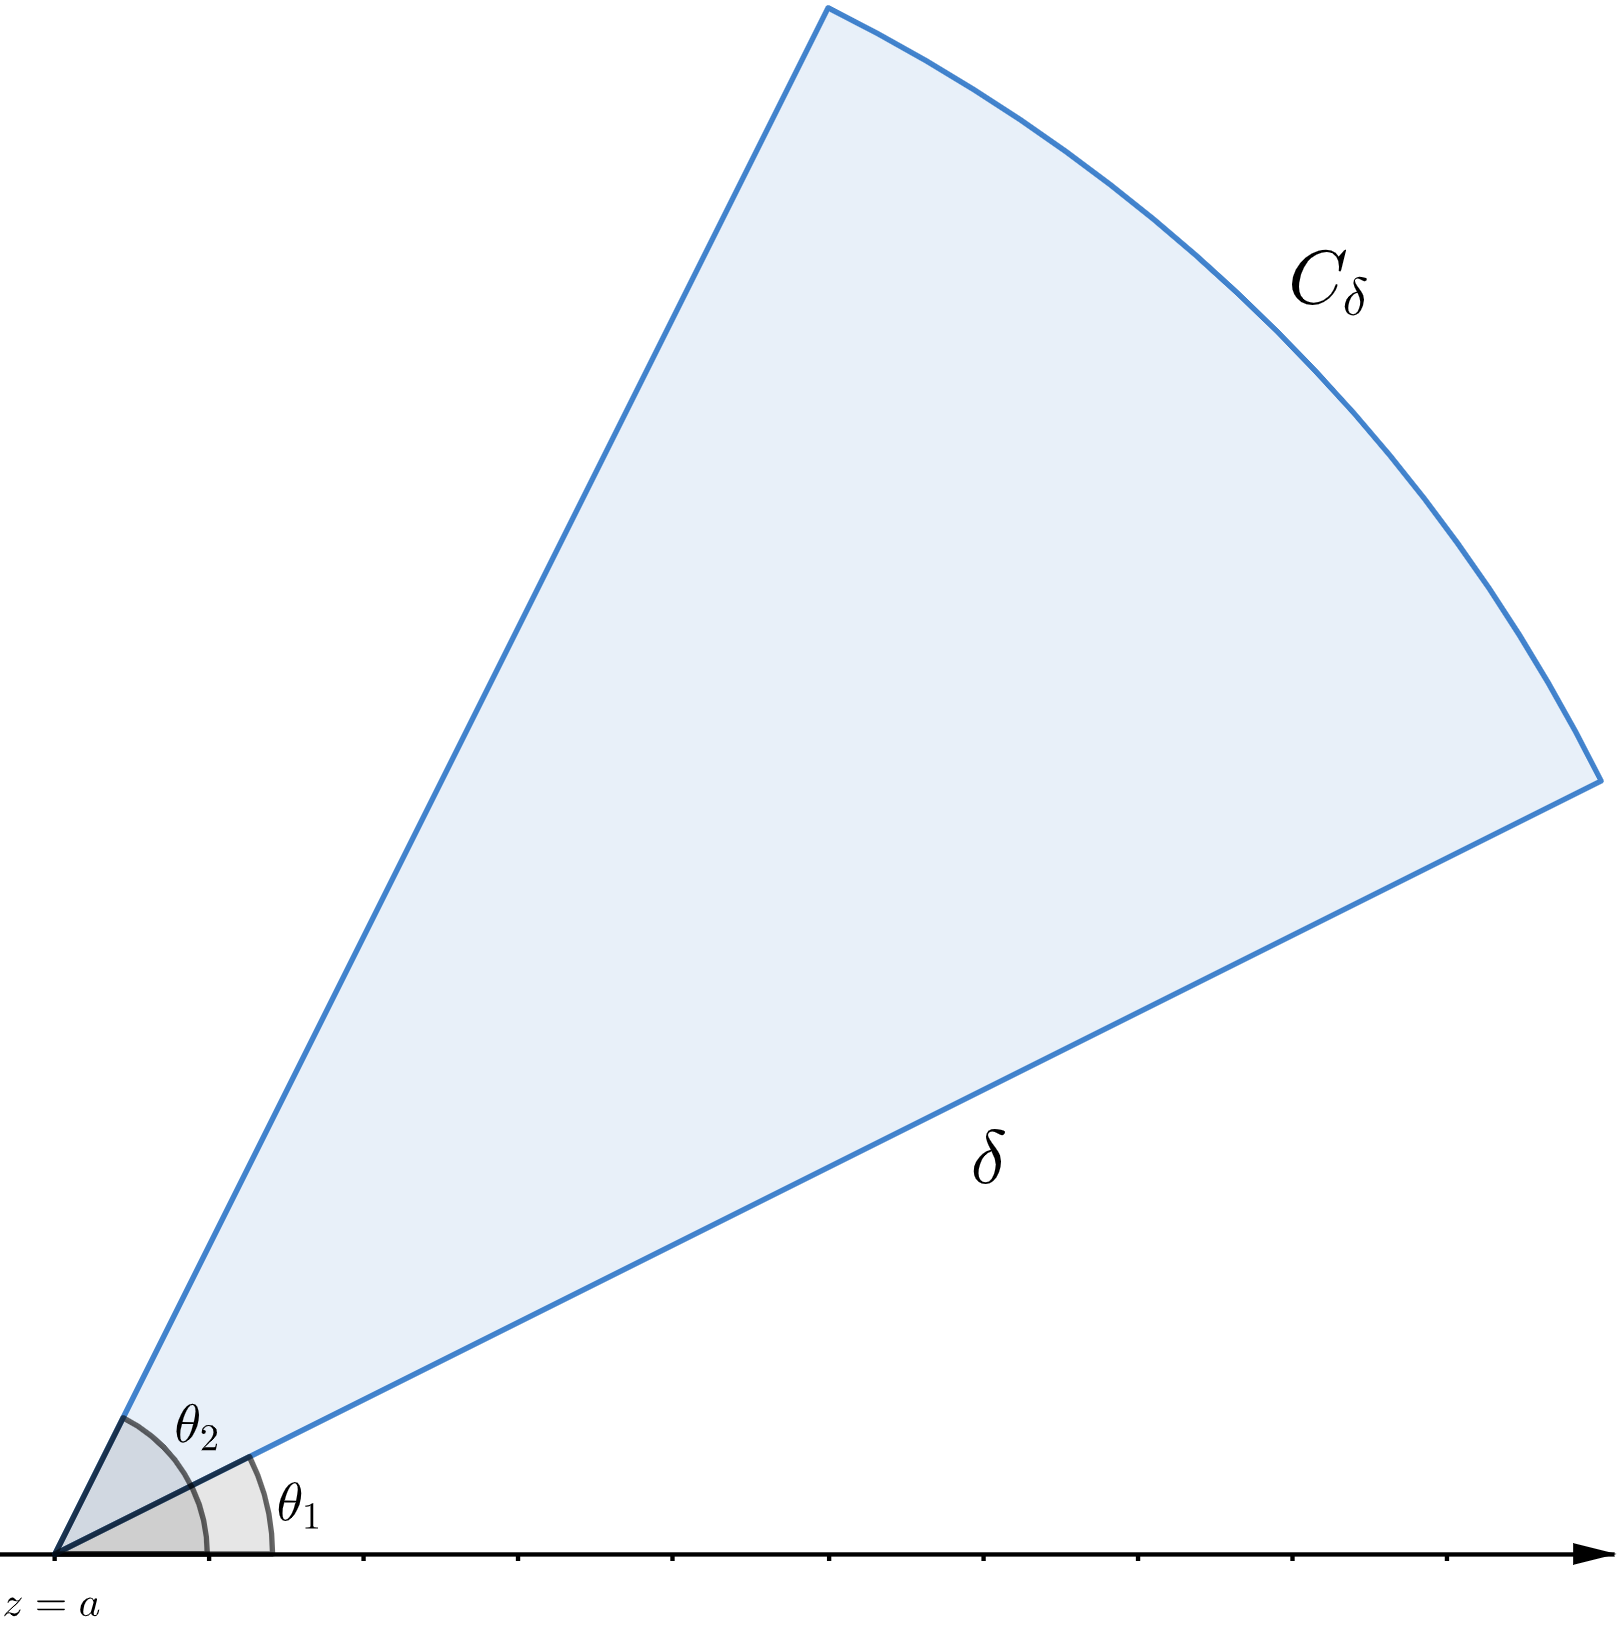
\includegraphics[width=0.9\textwidth]{SmallArc.png}
                \caption{小圆弧}
                \label{fig:small_arc}
            \end{minipage}
            \begin{minipage}[t]{0.48\textwidth}
                \centering
                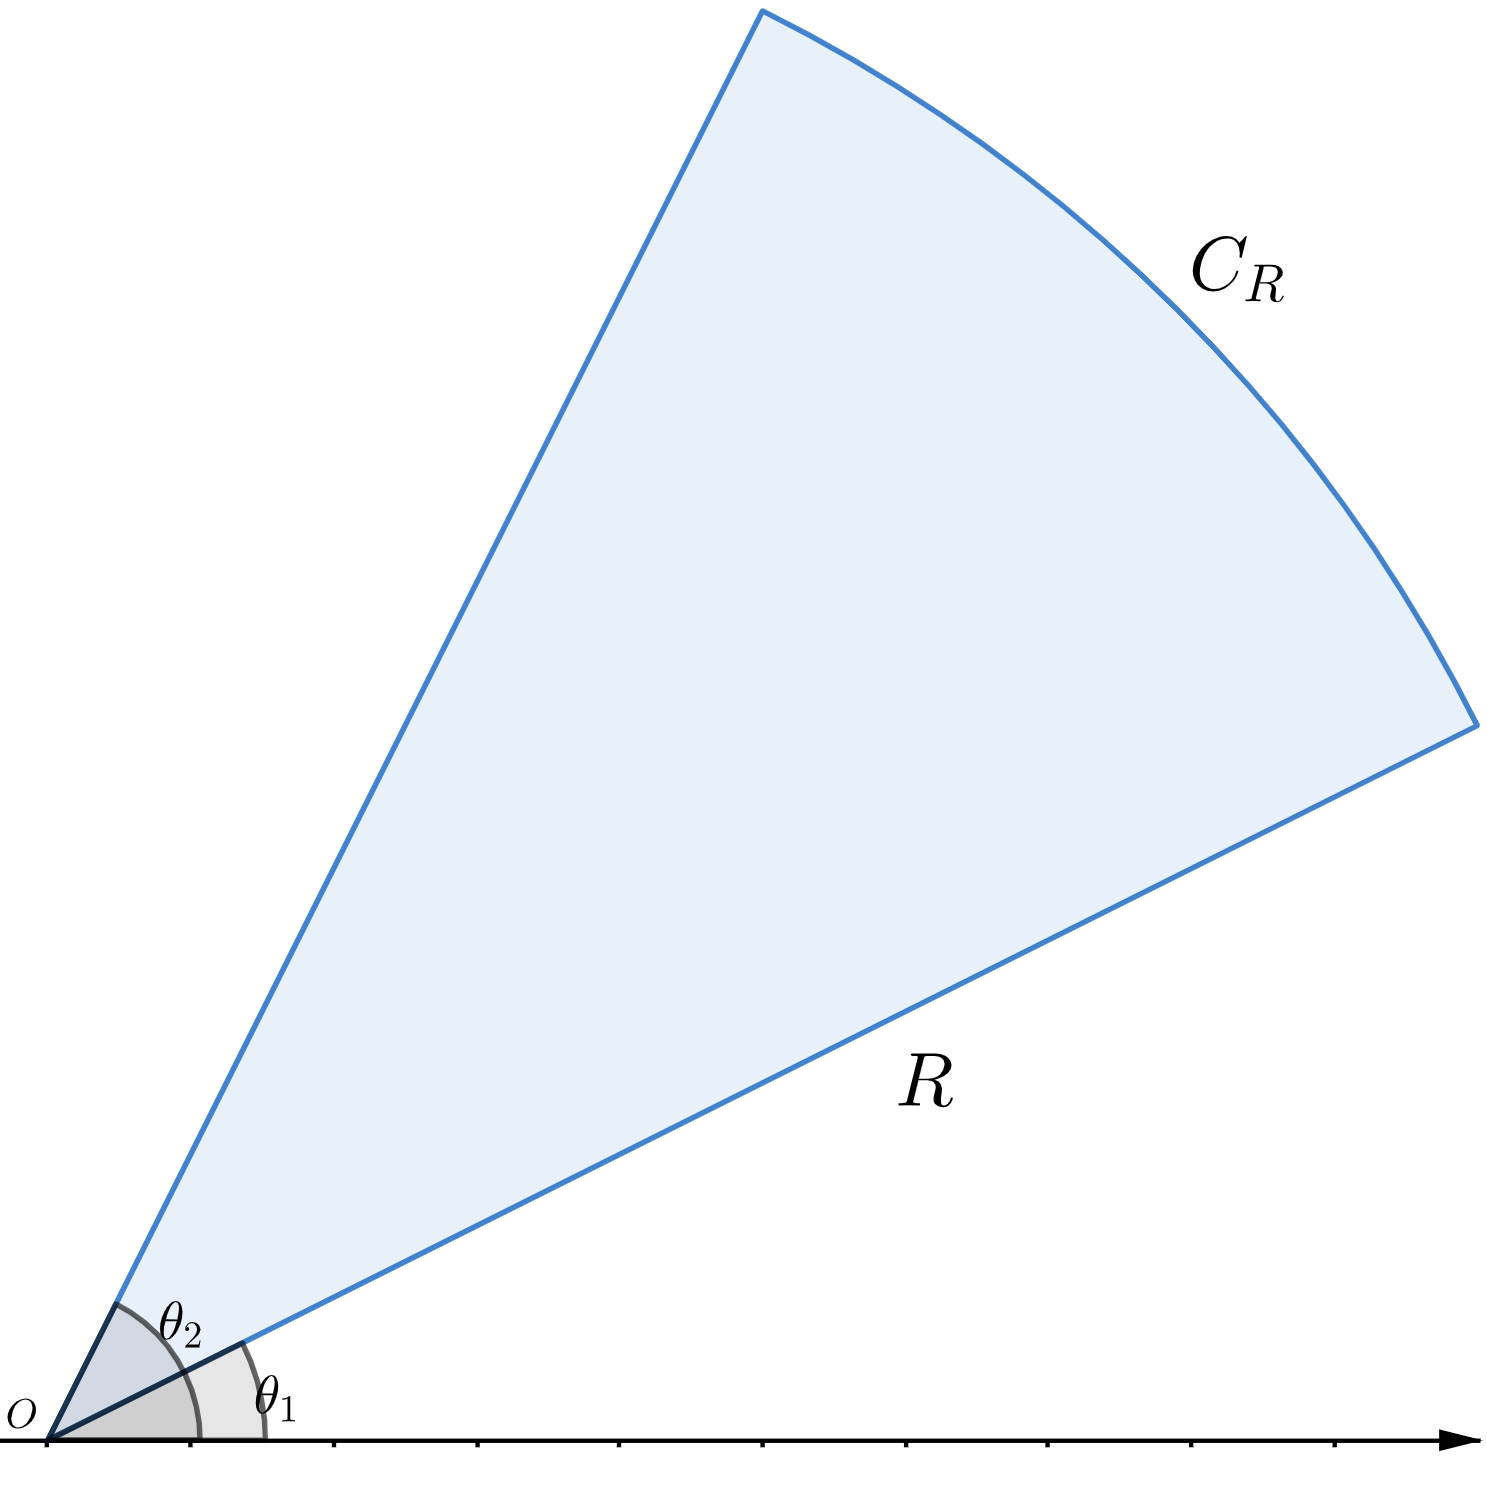
\includegraphics[width=0.9\textwidth]{LargeArc.png}
                \caption{大圆弧}
                \label{fig:large_arc}
            \end{minipage}
        \end{figure}

        \begin{lemma}
            \label{lem:large_arc_lemma}
            大圆弧引理:与小圆弧引理相似,若函数$f(z)$在$\infty$点的领域内连续,且在$\theta_1 \leq \arg{z} \leq \theta_2$区域内时,
            有$\lim_{|z| \to \infty}zf(z) \to K$,则
            \begin{align*}
                \lim_{R \to \infty}\int_{C_R}f(z)dz = iK(\theta_2 - \theta_1)
            \end{align*}
            式中$C_R$是以原点为圆心、$R$为半径、角度为$\theta_2 - \theta_1$的圆弧,
            $|z| = R,\,\theta_1 \leq \arg{z} \leq \theta_2$,如图\ref{fig:large_arc}所示.
        \end{lemma}

    \subsection{柯西积分公式}
        \begin{theorem}[Cauchy积分公式]\label{thm:cauchy_integral_formula}
            (Cauchy Integral Formula,简称CIF)设函数$f:\mathbbm{C} \to \mathbbm{C}$
            在闭合曲线$C$上解析,则对$C$内任一个点$z = z_0$,都有
            \begin{align*}
                \label{eq:cauchy_integral_formula}
                f(z_0) = \frac{1}{2 \pi i}\oint_{C}\frac{f(z)}{z - z_0}dz
            \end{align*}
        \end{theorem}

        \begin{example}
            使用CIF求出下列三式的值
            \begin{align*}
                &I_1 = \oint_{C_1}\frac{z^2dz}{(z^2+3)^2(z-i)},
                \quad I_2=\oint_{C_2}\frac{(z^2-1)dz}{(z-\frac{1}{2})(z^2-4)^3},\\
                &I_3=\oint_{C_3}\frac{e^{\frac{z}{2}}dz}{(z-i\pi)(z^2-20)^4},
            \end{align*}
            $C_1,\ C_2,\ C_3$分别为以原点为圆心,以$r_1=\dfrac{3}{2},\ r_2=1,\ r_3=4$为半径的圆.
        \end{example}
        \begin{solution}
            对$I_1$,我们令$f(z) = \dfrac{z^2}{(z^2+3)^2}$,易见$f$在$C_1$及其内点上解析,
            在$C$内选取$z_0 = i$,由$CIF$我们有:
            \begin{align*}
                I_1=\oint_{C_1}\frac{f(z)dz}{z-i}=2\pi i f(i)=2\pi i\frac{i^2}{(i^2+3)^2}=-i\frac{\pi}{2}.
            \end{align*}

            同理,对于$I_2$我们取$f(z) = \dfrac{z^2 - 1}{(z^2 - 4)^3},\ z_0 = i$.
            \begin{align*}
                I_2 = \oint_{C_2}\frac{f(z)dz}{z - \frac{1}{2}} = 2\pi i f(\frac{1}{2}) = \frac{32\pi}{1125}i.
            \end{align*}

            对于$I_3$我们取$f(z) = \frac{e^{z/2}}{(z^2 - 20)^4},\ z_0 = i\pi$.
            \begin{align*}
                I_3 = \oint_{C_3}\frac{f(z)dz}{z-i\pi}=2\pi i f(i\pi) = -\frac{2\pi}{(\pi^2+20)^4}.
            \end{align*}
        \end{solution}

    \subsection{解析函数的高阶导数}
        我们先将$CIF$写成如下形式:
        \begin{align*}
            f(z) = \frac{1}{2\pi i}\int_C \frac{f(\xi)d\xi}{\xi - z}.
        \end{align*}

        \begin{theorem}[解析函数的高阶导数]\label{thm:analytic_function_derivative}
            对上式求$n$阶导我们可以得到解析函数的$n$阶导公式:
            \begin{align*}
                f^{(n)}(z) = \frac{d^n f}{dz^n} = \frac{n!}{2\pi i}\oint_C \frac{f(\xi)d\xi}{(\xi - z)^{n + 1}}
            \end{align*}
        \end{theorem}

        我们将如下形式的积分称为柯西型积分:$$\oint_C \frac{g(\xi)d\xi}{p(\xi)}$$
        其中$p(z)$为关于$\xi$的多项式,即$p(\xi) = a_n(\xi - z_1)(\xi - z_2)\cdots(\xi - z_n)$.
        柯西型积分的求解有十分甚至九分简单,简要来说就是找处在$C$内的奇点,并确定函数$f(\xi)$和阶数,
        通过下例我们可以更加直观的理解柯西型积分的求解过程.
        \begin{example}
            求解柯西型积分
            \begin{align*}
                \oint_{|z + 1| = 1}\frac{dz}{(z + 1)^2(z - 2)}.
            \end{align*}
        \end{example}
        \begin{solution}
            $z = -1$为$|z + 1| < 1$内的一个奇点,$\dfrac{1}{z - 2}$在$|z + 1| < 1$内解析,
            由定理\ref{thm:analytic_function_derivative},我们有
            \begin{align*}
                \oint_{|z + 1| = 1}\frac{\frac{1}{z - 2}}{(z + 1)^2}dz = 2\pi i\left( \frac{1}{z - 2} \right)'\Bigg|_{z=-1} = -\frac{2}{9}\pi i
            \end{align*}
        \end{solution}

    \chapter{无穷复数项级数}
\begin{introduction}
    \item 复数项级数
    \item 复幂级数
    \item Taylor级数
    \item Laurent级数
    \item 解析延拓
\end{introduction}

\section{复数项级数}
    \subsection{复数项级数}
    复数项级数和实数项级数完全类似,直接快进到审敛法(

    \subsection{复数项级数的审敛定理}
    这里给出复数项级数的审敛定理.
    \begin{enumerate}
        \item 比值判别法\\
            若$\exists N \subset \mathbbm{N}$,对$\forall n > N$,都有
            $|u_n| < v_n$,并且$\sum_{n = 0}^{\infty}v_n$收敛,则$\sum_{n=0}^{\infty}|u_n|$收敛,即$\sum_{n=0}^{\infty}u_n$绝对收敛.
            若$u_n>v_n>0$,且$\sum_{n=0}^{\infty}v_n$发散,则$\sum_{n=0}^{\infty}|u_n|$发散.
        \item 比值判别法\\
            若存在与$n$无关的常数$\rho$,使得$\left|\dfrac{u_{n+1}}{u_n}\right|<\rho<1$,则级数$\sum_{n=0}^{\infty}u_n$绝对收敛;
            若$\left|\dfrac{u_{n+1}}{u_n}\right|>\rho>1$,则级数发散.
        \item $d'Alembert$判别法\\
            若$\varlimsup_{n\to\infty}|\dfrac{u_{n+1}}{u_n}|<1$,则级数$\sum_{n=0}^{\infty}u_n$绝对收敛;
            若$\varliminf_{n\to\infty}|\dfrac{u_{n+1}}{u_n}|>1$,则级数发散.
        \item $Cauchy$判别法\\
            同$d'Alembert$判别法,只需将$\varlimsup_{n\to\infty}|\dfrac{u_{n+1}}{u_n}|$和$\varliminf_{n\to\infty}|\dfrac{u_{n+1}}{u_n}|$
            均更换为上极限$\varlimsup{{|u_n|}^{1/n}}$.\\
            若$d'Alembert$判别法和$Cauchy$判别法中的两式均为$1$,我们可以使用下面的$Gauss$判别法.
        \item $Gauss$判别法\\
            若$\lim_{n\to\infty}|\dfrac{u_{n+1}}{u_n}|=1$,我们将邻项比值写成如下形式:
            \begin{align*}
                \frac{u_n}{u_{n+1}}=1+\frac{\mu}{n}+O(n^{-\lambda})
            \end{align*}
            这里我们一般通过$Taylor$展开得到.其中$\mu=a+ib,\ \lambda > 1$,若$a>1$,则级数绝对收敛,反之发散.
    \end{enumerate}
    \begin{example}
        判断级数$\sum_{n=1}^{\infty}\dfrac{i^n}{n^\alpha}\,(\alpha>0)$的收敛性和绝对收敛性.
    \end{example}
    \begin{solution}
        我们可以看到,$\sum_{n=1}^{\infty}|\dfrac{i^n}{n^\alpha}|=\sum_{n=1}^{\infty}\dfrac{1}{n^\alpha}$,
        这就是实数项级数中的$p$级数,所以当$\alpha\leq 1$时级数发散,反之绝对收敛.这里我们使用$Gauss$判别法得到相同结论:
        \begin{align*}
            \frac{c_n}{c_{n+1}}=\frac{1/n^\alpha}{1/(n+1)^\alpha}=\left( 1+\frac{1}{n} \right)^\alpha=1+\frac{\alpha}{n}+O\left(\frac{1}{n^2}\right)
        \end{align*}
        当$\alpha \leq 1$时级数发散,反之收敛.
    \end{solution}

\section{复幂级数}
    \subsection{复幂级数的定义和性质}
        \begin{definition}[复幂级数]\label{def:complex_power_series}
            我们将形如$\sum_{k=0}^{\infty}(z-z_0)^k$的复函数项级数称为复幂级数.
        \end{definition}

        \begin{proposition}
            若幂级数$\sum_{k=0}^{\infty}a_k(z - z_0)^k$在点$z_1=\neq z_0$处收敛,则该级数在$|z-z_0|<|z_1-z_0|$处均收敛;
            同样地,若幂级数$\sum_{k=0}^{\infty}b_k(z - z_0)^{(-k)}$在点$z_2=\neq z_0$处收敛,则该级数在$|z-z_0|>|z_2-z_0|$处均收敛
        \end{proposition}

    \subsection{复幂级数的收敛半径计算}
        这部分和实幂级数的计算方法完全一样,但是在计算时要时刻提醒自己算的是复数.
        \begin{enumerate}
            \item 由$Cauchy$判别法,我们可以得到$Cauchy-Hadamard$公式:
                \begin{align}
                    R=\varliminf_{n\to\infty}\left|\frac{1}{c_n}\right|^{1/n}
                \end{align}
            \item 由$d'Alembert$判别法,我们可以得到:
                \begin{align}
                    R=\lim_{n\to\infty}\left|\frac{c_n}{c_{n+1}}\right|
                \end{align}
        \end{enumerate}
        \begin{remark}
            $Cauchy-Hdamard$公式在任意条件下均成立,但$d'Alembert$公式要求有$\lim_{n\to\infty}|c_n/c_{n+1}|$存在.
            求收敛半径时一般先用后者,行不通再使用前者.使用前者时一般要用到重要极限,请牢牢记住$\lim_{f(x)\to\infty}\left(1+\dfrac{1}{f(x)}\right)^{f(x)}=e$.
        \end{remark}

\section{Taylor级数}
    \subsection{Taylor级数的定义}
        \begin{definition}[Taylor级数]\label{def:taylor_series}
            设$f(z)$在圆域$C$内解析,$z_0$为$C$内任一点,则函数$f(z)$可以展开为幂级数形式.
            \begin{align}
                f(z)=f(z_0)+f'(z_0)(z-z_0)+\cdots
                =\sum_{n=0}^{\infty}\dfrac{f^{(n)}(z_0)}{n!}(z-z_0)^n
            \end{align}
        \end{definition}
        \begin{definition}[Maclaurin级数]\label{def:maclaurin_series}
            这里如果取$z_0=0$,我们可以得到$Maclaurin$级数.
            \begin{align*}
                f(z)=f(0)+f'(0)z+\cdots=\sum_{n=0}^{\infty}\frac{f^{(n)}(0)}{n!}z^n
            \end{align*}
        \end{definition}

    \subsection{重要的Taylor级数}
        这部分请务必牢记,这些$Taylor$级数(都是在$z_0=0$点展开)在计算中会频繁用到,这里建议把每一个都自己手推一遍.
        \begin{enumerate}
            \item $e^z = \sum\dfrac{z^n}{n!},\ (|z|<\infty)$
            \item $\dfrac{1}{1-z}=\sum z^n,\ (|z|<1)$
            \item $\dfrac{1}{1+z}=\sum (-1)^n z^n,\ (|z|<1)$
            \item $\sin{z}=\sum(-1)^n\dfrac{z^{2n+1}}{(2n+1)!},\ (|z|<\infty)$
            \item $\cos{z}=\sum(-1)^n\dfrac{z^{2n}}{(2n)!},\ (|z|<\infty)$
            \item $\ln{(1+z)}=\sum(-1)^n\dfrac{z^{n+1}}{n+1},\ (|z|<1)$
            \item $(1+z)^\alpha=\sum\dfrac{\alpha(\alpha-1)\cdots(\alpha-n+1)}{n!}z^n=\sum\dbinom{\alpha}{n}z^n,\ (|z|<1)$
        \end{enumerate}

        \begin{note}
            这里补充一下普遍二项式的定义.
            \begin{align*}
                \binom{\alpha}{n}=\frac{\alpha(\alpha-1)\cdots(\alpha-n+1)}{n!}
            \end{align*}
        \end{note}

\section{Laurent级数}
    \subsection{Laurent级数的定义}
        \begin{figure}
            \centering
            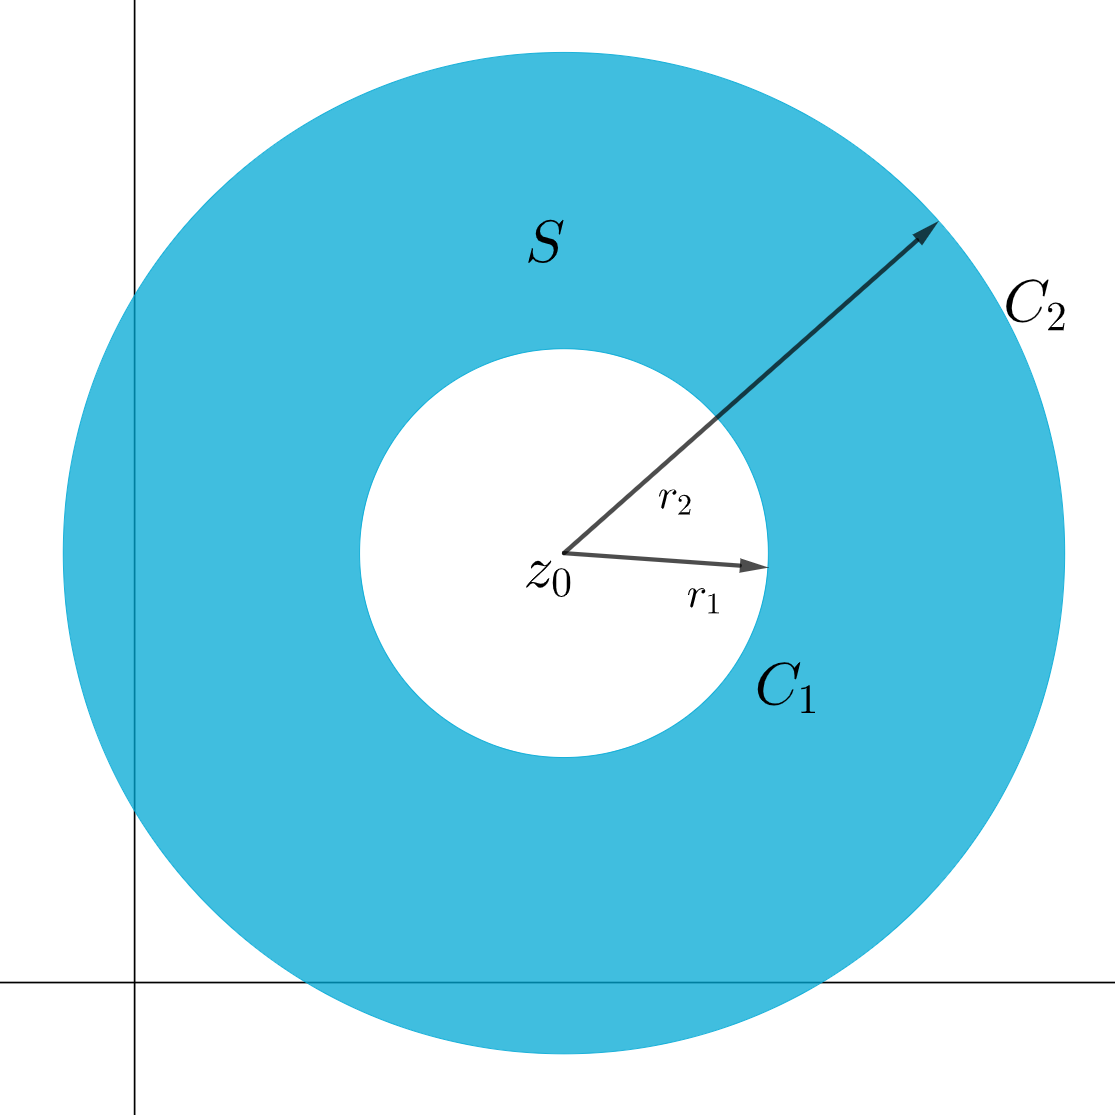
\includegraphics[width=0.5\textwidth]{AnnularRegion.png}
            \caption{展开为$Laurent$级数的函数解析区域}
            \label{fig:Laurent_series}
        \end{figure}
        \begin{definition}[Laurent级数]\label{def:laurent_series}
            如图\ref{fig:Laurent_series}所示,设$f(z)$在圆环$S$内单值解析,$z$为$S$内任一点,则函数$f(z)$可以展开为幂级数形式.
            \begin{align*}
                f(z)=\sum_{n=-\infty}^{\infty}a_n(z-z_0)^n,\quad a_n=\frac{1}{2\pi i}\oint_{C}\frac{f(\xi)}{(\xi-z_0)^{n+1}}d\xi
            \end{align*}
        \end{definition}
        函数$f(z)$在内圆$C_1$内不解析,但注意$f(z)$在点$z_0$上可能解析也可能不解析.

        $Laurent$级数有两部分,其中正幂项在外圆$C_2$内内闭一致收敛,负幂项在内圆$C_1$外绝对收敛.其中负幂项被称为$Laurent$级数的主要部分,当$Laurent$级数没有
        负幂项时,它就是$Taylor$级数.


    \subsection{Laurent级数的计算}
        废话不多说,直接上例题.
        \begin{example}
            将函数$f(z)=\dfrac{2+3z}{z^2+z^3}$在$z=0$点处写成$Laurent$级数的形式.
        \end{example}
        \begin{solution}
            我们有:
            \begin{align*}
                f(z)&=\frac{1}{z^2}\left(\frac{2+3z}{1+z}\right)=\frac{1}{z^2}\left(3-\frac{1}{1+z}\right)
                =\frac{1}{z^2}\left(3-\sum_{n=0}^{\infty}(-1)^nz^n\right)\\
                &=\frac{1}{z^2}(3-1+z-z^2+z^3-\cdots)=\frac{2}{z^2}+\frac{1}{z}-1+z-z^2+\cdots
            \end{align*}
            该级数在$|z|<1$上收敛.
        \end{solution}

        \begin{example}
            讨论函数$f(z)=1/(4z-z^2)$的$Laurent$展开.
        \end{example}
        \begin{solution}
            该函数有两个奇点$z=0,\,z=4$.所以我们将该函数分别在$z=0$处和$z=\infty$处展开.

            当$|z|<4$时,我们有$|z/4|<1$:
            \begin{align*}
                f(z)=\frac{1}{4z}\left(\frac{1}{1-z/4}\right)=\frac{1}{4z}\sum_{n=0}^{\infty}\left(\frac{z}{4}\right)^n=\sum_{n=0}^{\infty}4^{-n-1}z^{n-1}=\sum_{n=-1}^{\infty}4^{-n-2}z^n.
            \end{align*}

            当$|z|>4$时,我们有$|4/z|>1$(此时是在点$z=\infty$处展开):
            \begin{align*}
                f(z)=-\frac{1}{z^2}\left(\frac{1}{1-4/z}\right)=-\frac{1}{z^2}\sum_{n=0}^{\infty}4^nz^{-n}=-\sum_{-\infty}^{-2}4^{-n-2}z^{n}.
            \end{align*}
        \end{solution}

        从上面这俩例题我们能看到求解$Laurent$级数和使用间接法求解$Taylor$级数十分类似,只是需要注意自变量的取值范围.

    \subsection{奇点的分类}
        定义\ref{def:singular_point}将奇点定义为函数$f$不解析的点,实际上奇点还可以细分为
        在其任一空心邻域上均解析的孤立奇点和在其任一空心邻域上都有其他奇点的非孤立奇点.
        孤立奇点根据函数的$Laurent$级数又可以分为可去奇点、极点和本性奇点.

        \begin{remark}
            非孤立奇点一般出现在多值函数中,我们将在第三章留数定理中再讨论非孤立奇点.
        \end{remark}

        \begin{enumerate}
            \item 可去奇点\\
                级数展开式不含负幂项.$f(z)=\sum_{n=0}^{\infty}a_n(z-z_0)^n$
            \item 极点\\
                级数展开式含有有限个负幂项,特别的,如果级数展开式含有$m,\ (m\neq \infty)$个负幂项,则称为$m$阶极点.$f(z)=\sum_{n=-m}^{\infty}a_n(z-z_0)^n$
            \item 本性奇点\\
                级数展开式含有无穷个负幂项.$f(z)=\sum_{-\infty}^{\infty}a_n(z-z_0)^n$
        \end{enumerate}

        \begin{note}
            当我们讨论$f(z)$的无穷远点时,我们可以令$z=1/t$,此时点$t=0$的性质就是点$z=\infty$处的性质.
        \end{note}


\section{解析延拓}

    \subsection{解析延拓的定义}
        \begin{definition}[解析延拓]\label{def:analytic_continuation}
            设有函数$f_1,\,f_2:\mathbbm{C}\to\mathbbm{C}$,分别在区域$G_1,\,G_2$上解析,且$G_1\cap G_2=g\neq \varnothing$.如果有$\forall z\in g,\ f_1(z)\equiv f_2(z)$,
            则称$f_1$是$f_2$在$G_1$中的解析延拓,$f_2$是$f_1$在$G_2$中的解析延拓.
        \end{definition}

    \subsection{解析延拓的应用}
        使用复分析处理问题的时候,我们就可以先在较小区域内定义出复变函数,再使用解析延拓将其拓展到我们想要使用的地方,
        黎曼$\zeta $函数和$\Gamma$函数就是通过解析延拓得到的.我们的课程并没有详细讲解解析延拓,也不会考察,但是解析延拓在后续数学物理的学习中用处挺大,有兴趣很建议详细学习相关内容.


\end{document}